\section{Constructive Heuristics}
In Combinatorial Optimization every solution $x$ is a subset of the ground set $B$.\\

Essentially we want to add an element at a time to an empty subset until it doesn't make sense anymore to have new elements.\\

A constructive heuristic \textbf{updates a subset} $x^{(t)}$ step by step
\begin{enumerate}
	\item \textbf{start} from an \textbf{empty subset}: $x^{(0)} = \emptyset$ (obviously a subset of any optimal solution)
	\item \textbf{stop} when a \textbf{termination condition} holds (the following subsets cannot be optimal solutions, there are no more elements to be added that lead to an optimal solution)
	\item \textbf{select} the "\textbf{best}" element $i^{(t)} \in B \setminus x$ among the "acceptable" ones (parameter which needs to be determined) at the current step $t$ (try and keep $x^{(t)}$ within a feasible and optimal solution)
	\item \textbf{add} $i^{(t)}$ to the \textbf{current subset} $x^{(t)}: \, x^{(t+1)} := x^{(t)} \cup \{i^{(t)}\}$ (the selection can never be undone!)
	\item go \textbf{back to point 2}
\end{enumerate}
Such processes admit a nice modeling tool.\\

\newpage

\subsection{Construction Graph}
Every construction heuristic $A$ defines a \textbf{construction graph}
\begin{itemize}
	\item the \textbf{node set} $\mathcal{F}_A \subseteq 2^B$ (\textbf{search space}) is the collection of all subsets $x \subseteq B$ acceptable for $A$
	\item the \textbf{arc set} is the collection of all pairs $(x, x \cup \{i\})$ such that $x \in \mathcal{F}_A$, $i \in B \setminus x$ and $x \cup \{i\} \in \mathcal{F}_A$ (connects $x$ with $x$ plus one element). The arcs represent the elementary extensions of the acceptable subsets
\end{itemize}

It's a directed graph in which the nodes compose the search space, dependent on $A$, and the arcs link all the element of the search space to every element with a cardinality of one more. Essentially the nodes are all the possible subsets, while the arcs represent all the possible connections (additions of elements) for each node (subset).\\

The construction graph is by definition \textbf{acyclic}.\\

Each possible execution of $A$ is a \textbf{maximal path of the construction graph}
\begin{itemize}
	\item \textbf{from} the empty subset $x = \emptyset$
	\item to a subset $x$ that \textbf{cannot be acceptably extended} (and hopefully a feasible solution)
\end{itemize}
$$ \Delta^+_A (x) = \left\{i \in B \setminus x : \, x \cup \left\{i\right\} \in \mathcal{F}_A \right\} = \emptyset $$

\newpage

\paragraph{Example}
\begin{center}
	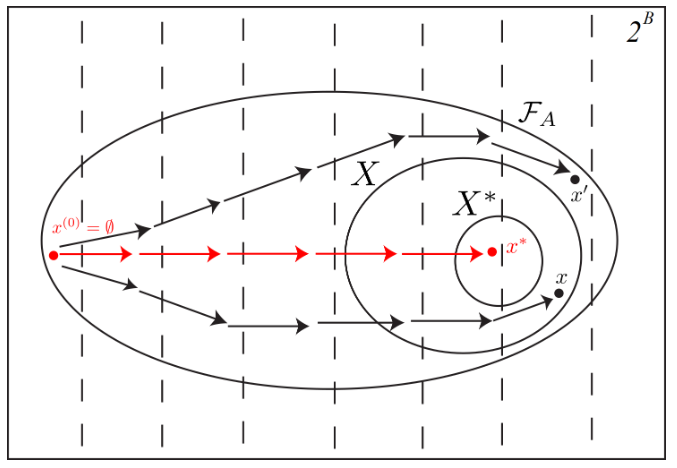
\includegraphics[width=0.8\columnwidth]{img/CGraph1}
\end{center}
The algorithm visits a \textbf{sequence of subsets} $\emptyset = x^{(0)} \subset \, ... \, \subset x^{(t_f)}$ terminating
\begin{itemize}
	\item in an \textbf{optimal solution} $x^\ast \in X^\ast$ (Example: MST problem, both with $\mathcal{F}_{Kruskal}$ and $\mathcal{F}_{Prim}$)
	\item in a \textbf{nonoptimal feasible solution} $x \in X$ (Example: KP, MDP, etc...)
	\item in an \textbf{unfeasible subset} $x'$ (Example: TSP on a noncomplete graph)
\end{itemize}

\newpage

\subsubsection{Termination condition} 
A constructive heuristic $A$ \textbf{terminates} when
\begin{itemize}
	\item the current \textbf{subset} $x^{(t)}$ has \textbf{no outgoing arc}
	$$ \Delta^+_A \left(x^{(t)}\right) = \left\{i \in B \setminus x^{(t)} : \, x^{(t)} \cup \left\{i\right\} \in \mathcal{F}_A \right\} = \emptyset $$
	$\Delta^+_A \left(x^{(t)}\right)$ represents the subset of the ground set that can be added in $x^{(t)}$ in an acceptable manner for algorithm $A$ (what I can add to our solution).\\
	
	\item that is, \textbf{extending} $x^{(t)}$ implies to \textbf{leave the search space} $\mathcal{F}_A$
	$$ x^{(t)} \cup \left\{i\right\} \notin \mathcal{F}_A \text{ for each } i \in B \setminus x^{(t)}$$
\end{itemize}

There is no arc going out of the node in the construction graph.\\

The algorithm returns the \textbf{best solution visited} during the execution (usually the last one).\\

Different behaviors are possible
\begin{itemize}
	\item sometimes \textbf{all} visited \textbf{subsets} are \textbf{feasible} (e.g., KP)
	\item often the \textbf{last subset} is the only \textbf{feasible} solution
	\item $x^{(t)}$ could even \textbf{move in and out} of $X$ (or $X^\ast$; but this is uncommon)
	\item the path \textbf{can visit or not} $X$ and $X^\ast$
\end{itemize}

\newpage

\subsubsection{Definition of the construction graph}
Ideally, the \textbf{search space} $\mathcal{F}_A$ should \textbf{include}
\begin{itemize}
	\item the \textbf{empty subset}: $\emptyset \in \mathcal{F}_A$ ($A$ starts from $\emptyset$)
	\item all \textbf{feasible solutions}: $X \subseteq \mathcal{F}_A$ (maybe excluding provably nonoptimal solutions)
	\item \textbf{only subsets accessible from} $\emptyset$ (inaccessible subsets are useless)
\end{itemize}

Using $\mathcal{F}_A$ requires a \textbf{fast inclusion test} to answer the decision problem:
\begin{itemize}[label*=]
	\item "is subset $x^{(t)}$ acceptable?" ($x^{(t)} \in \mathcal{F}_A$?)
\end{itemize}
or at least a \textbf{fast update test}: if $x^{(t)} \in \mathcal{F}_A$, is $x^{(t)} \cup \{i\} \in \mathcal{F}_A$? \\

$\mathcal{F}_A = \left\{x' \subseteq B : \, \exists x \in X : \, x' \subseteq x\right\}$ (subsets of feasible solutions, i.e. \textbf{partial solutions}) is a natural candidate, but its \textbf{inclusion test}
\begin{itemize}[label*=]
	\item "is subset $x^{(t)}$ a partial solution?" ($\exists x \in X : \, x^{(t)} \subseteq x$?)
\end{itemize}
\textbf{generalizes} the feasibility problem ($\exists x \in X : \, \emptyset \subseteq x$?)
\begin{itemize}[label*=]
	\item "is there any feasible solution?" ($\exists x \in X$?)
\end{itemize}
and could be $\np$-complete. In that case, one needs to \textbf{relax the search space}; include other subsets which may lead to more sub-optimal solutions, while making the acceptability test easier.\\

Including a partial solution is like asking "is there a solution that includes this subset?" and could be an $\np$-complete problem, not always polynomial.\\

If the \textbf{objective function} can be extended from $X$ to $\mathcal{F}_A$, it looks natural to use the objective function as the \textbf{selection criteria}
$$ \phi_A (i,x) = f \left(x \cup \left\{i\right\} \right)$$

\newpage

\paragraph{Examples of search spaces:} The search space $\mathcal{F}_A$ may include:
\begin{itemize}
	\item \textbf{All feasible solutions}
	$$ \mathcal{F}_A = X $$
	In the KP, all subsets of feasible weight.\\
	
	\item \textbf{All partial (and all feasible) solutions}
	$$ \mathcal{F}_A = \bigcup_{x \in X} 2^x $$
	In the MDP, all subsets of at most $k$ points.\\
	In Kruskal's algorithm for the MSTP, all spanning forests.\\
	
	\item \textbf{Only some special promising partial solutions}
	$$ \mathcal{F}_A \subset \bigcup_{x \in X} 2^x $$
	In Prim's algorithm for the MSTP, all trees spanning a given vertex.\\
	
	\item \textbf{Some special subsets not sufficient to guarantee feasibility}
	$$ \mathcal{F}_A \supset \bigcup_{x \in X} 2^x $$
	In the TSP, all subsets of arcs not including branching and sub-tours.\\
\end{itemize}

\newpage

\subsection{Effectiveness and Efficiency}
A constructive algorithm $A$ finds the optimum when at \textbf{each step} $t$ the current subset $x^{(t)}$ \textbf{is included} in at least one \textbf{optimal solution}. An exact algorithm always keeps an open way to an optimal solution.\\
This property holds in $x^{(0)} = \emptyset$, but is usually lost at some step $t$,\\

A constructive algorithm performs at \textbf{most} $n = |B|$ \textbf{steps} (can't add more element than the whole ground set) consisting of 
\begin{enumerate}
	\item the \textbf{construction} of $\Delta_A^+ (x)$
	\item the \textbf{evaluation} of $\phi_A (i,x)$ for each $i \in \Delta_A^+(x)$
	\item the \textbf{selection} of the element $i$ minimizing $\phi_A (i,x)$
	\item the \textbf{update} of $x$ (and auxiliary data structures)
\end{enumerate}
In general, the \textbf{complexity} is a \textbf{polynomial} of rather low order, dominated by the first two components
$$ T_A (n) \in O\left(n \left(T_{\Delta_A^+} (n) + T_{\phi_A} (n)\right)\right) $$

\newpage

\subsection{General features}
Constructive algorithms
\begin{itemize}
	\item are \textbf{intuitive}
	\item are \textbf{simple} to design, analyze and implement
	\item are \textbf{very efficient} (usually low complexity)
	\item have a \textbf{strongly variable effectiveness}; they can range from providing an optimal solution on some problem to not even guaranteeing a feasible solution; on most problems they provide solutions of extremely variable quality, often low
\end{itemize}
It is fundamental to \textbf{study the problem} before the algorithm.\\

\paragraph{When are they used?} Constructive algorithms are used
\begin{itemize}
	\item when they \textbf{provide} the \textbf{optimal solution}
	\item when the \textbf{execution time} must be \textbf{very short} 
	\item when the \textbf{problem} has a \textbf{huge size} or requires heavy computation 
	\item as a \textbf{component for other algorithms}, for example as
	\begin{itemize}
		\item \textbf{starting phase} for exchange algorithms 
		\item \textbf{basic procedure} for recombination algorithms
	\end{itemize}
\end{itemize}

\paragraph{Remarkable case:} A particularly remarkable case is that in which
\begin{itemize}
	\item the \textbf{objective function} is \textbf{extended} from $X$ to $\mathcal{F}_A$
	\item the \textbf{selection criteria is the objective function}
	$$ \phi_A (i,x) = f\left(x \cup \left\{i\right\}\right) $$
\end{itemize}
This means that instead of minimizing the selection criteria (which is generic) I use the value of the objective function. It's a greedy algorithm, sometimes can be a good idea.\\

\newpage

\subsection{Examples}
\subsubsection{The Fractional Knapsack Problem (FKP)}
Select from a set of \textbf{objects of identical volume} a \textbf{maximum value subset} which could be contained in a \textbf{knapsack of limited capacity} (same as the KP but all the objects have the same volume).\\

In the FKP the capacity simply imposes a \textbf{cardinality constraint}: the feasible solutions are those with $|x| \leq \lfloor V / v \rfloor$

\begin{algorithm}
	\caption{Algorithm $GreedyFKP(i)$}
	\begin{algorithmic}
		\STATE $x := \emptyset$; $x^\ast := \emptyset$;
		\IF{$x \in X$} 
		\STATE $f^\ast := f(x)$ ;
		\ELSE
		\STATE $f^\ast := + \infty$;
		\ENDIF
		\WHILE{$|x| < \lfloor V/v \rfloor$}
		\STATE $i:= \arg \max_{i \in B \setminus x} \phi_i$;
		\STATE $x := x \cup \left\{i\right\}$;
		\IF{$x \in X$ and $f(x) > f^\ast$}
		\STATE $x^\ast := x$; $f^\ast := f(x)$;
		\ENDIF
		\ENDWHILE
		\RETURN ($x^\ast, f^\ast$)
	\end{algorithmic}
\end{algorithm}

\begin{itemize}
	\item Define $\mathcal{F}_A = X$: subset $x$ can be extended as long as $|x| < \lfloor V/v \rfloor$
	\item Any or no element of $B \setminus x$ extends $x$ feasibly ($\Delta_A (x) = B \setminus x$ or $\emptyset$)
	\item The objective function is additive, and therefore
	$$ f(x \cup \left\{i\right\}) = f(x) + \phi_i \implies \arg \max_{i \in B \setminus x} f(x \cup \left\{i\right\}) = \arg \max_{i \in B \setminus x} \phi_i $$
	\item The last subset visited is the best solution found
\end{itemize}
Just add objects until the cardinality is reached, add the most valuable one each time. Each solution is better than the previous one, since it's larger.\\

The algorithm always finds the optimal solution.\\

\newpage

\subsubsection{The Knapsack Problem} 
Select from a set of objects of \textbf{different volume} a maximum value subset which could be contained in a knapsack of limited capacity.\\

The algorithm is similar, the \textbf{differences} are:
\begin{itemize}
	\item The set of elements that can be added is the subset of items which do not exceed the residual capacity
	
	\item The termination condition must check that there is at least one element that can extend the current solution
\end{itemize}

\begin{algorithm}
	\caption{Algorithm $GreedyKP(i)$}
	\begin{algorithmic}
		\STATE $x := \emptyset$; $x^\ast := \emptyset$; $f^\ast := 0$
		\WHILE{$\exists i \in B \setminus x : \, v_i \leq V - \sum_{j \in x} v_j$}
		\STATE $i := \arg \max_{i \in B \setminus x : \, v_i \leq V - \sum_{j \in x} v_j} \phi_i$
		\STATE $x := x \cup \left\{i\right\}$
		\ENDWHILE
		\RETURN ($x, f(x)$)
	\end{algorithmic}
\end{algorithm}

Define $\mathcal{F}_A = X$: only some elements of $B \setminus x$ extend $x$ feasibly
$$ \Delta_A^+ (x) = \left\{i \in B \setminus x: \, \sum_{j \in x} v_j + v_i \leq V \right\} $$

The objective function is additive, and therefore
$$ f\left(x \cup \left\{i\right\}\right) = f(x) + \phi_i \implies \arg \max_{i \in \Delta_A^+ (x)} f\left(x \cup \left\{i\right\}\right) = \arg \max_{i \in \Delta_A^+ (x)} \phi_i $$

The last subset visited is the best solution found.\\

\newpage

\subsubsection{Traveling Salesman Problem}
Given a directed graph and a cost function defined on the arcs, find a \textbf{minimum cost circuit visiting all the nodes} of the graph.\\

Define $\mathcal{F}_A$ as the collection of all subsets of arcs that form no sub-tour and keep a degree $\leq 1$ in all nodes, (it is a superset of the partial solutions). The constructive algorithm add each time the cheapest arc among those in $\mathcal{F}_A$, until nothing can be added, that's the solution.\\

The selection criteria is the objective function (it is additive, therefore equivalent to the cost of the new arc).

\begin{algorithm}
	\caption{Algorithm $GreedyTSP(i)$}
	\begin{algorithmic}
		\STATE $x := \emptyset$; $x^\ast := \emptyset$;
		\STATE $f^\ast := + \infty$;
		\WHILE{$\Delta_A^+(x) \neq \emptyset$}
		\STATE $i := \arg \min_{i \in \Delta_A^+ (x)} c_i$;
		\STATE $x := x \cup \left\{i\right\}$;
		\ENDWHILE
		\IF{$x \in X$}
		\STATE $x^\ast := x$; $f^\ast := f(x)$;
		\ENDIF
		\RETURN ($x^\ast, f^\ast$)
	\end{algorithmic}
\end{algorithm}
Only the last subset visited can be feasible (if any!).\\

\newpage

\subsubsection{Maximum Diversity Problem}
Select from a set of points a subset of $k$ points with the \textbf{maximum sum of the pairwise distances}.\\

\begin{algorithm}
	\caption{Algorithm $GreedyMDP(i)$}
	\begin{algorithmic}
		\STATE $x := \emptyset$
		\WHILE{$|x| < k$}
		\STATE $i := \arg \max_{i \in B \setminus x} \sum_{j \in x} d_{ij}$
		\STATE $x := x \cup \left\{i\right\}$
		\ENDWHILE
		\RETURN ($x, f(x)$)
	\end{algorithmic}
\end{algorithm}

Define $\mathcal{F}_A$ as the set of all partial solutions.\\

The subset $x$ can be extended as long as $|x| < k$.\\

Any element of $B \setminus x$ extends $x$ in a feasible way.\\

The objective function is quadratic, and therefore
$$ f(x \cup \left\{i\right\}) = f(x) + 2 \sum_{j \in x} d_{ij} + d_{ii} \implies \arg \max_{i \in B \setminus x} \sum_{j \in x} d_{ij} $$

The last subset visited is the best (and only feasible) solution found.\\

\newpage

\subsubsection{Summary}
A constructive heuristic $A$ \textbf{finds}
\begin{itemize}
	\item The \textbf{optimum} when $\Delta_A^+ \left(x^{(t)}\right)$ and $\phi_A (i, x)$ guarantee that the current subset $x^{(t)}$ is \textbf{always included} in at least one \textbf{optimal solution}.\\
	
	\item A \textbf{feasible solution} when $\Delta_A^+ \left(x^{(t)}\right)$ guarantees that the current subset $x^{(t)}$ is \textbf{always included} in at least one \textbf{feasible solution}.\\
	
	\item A \textbf{general subset} when these \textbf{properties are lost} at some step $t$
\end{itemize}

An ideal constructive algorithm always keeps one open way to the optimal solution.\\

In practice, some of these properties is usually lost at some step of the algorithm.\\

\subsubsection{Relevant Features}
None of the above algorithms where able to find the optimum (except the FKP, examples not provided, but trust me).\\

What features allow a constructive algorithm to \textbf{find the optimum}? 
\begin{itemize}
	\item A \textbf{search space identical to the feasible region} ($\mathcal{F} = X$)? (No, because this holds for both the fractional and general KP)
	\item A \textbf{cardinality-constrained problem}? (It would explain failing on the KP, but not on the MDP and TSP)
	\item An \textbf{additive objective function}? (It does not explain failing on the TSP)
\end{itemize}

There is \textbf{no general characterization} of the problems solved exactly by constructive algorithms.\\

But there are characterizations for wide classes of problems.\\

\newpage

\subsection{The additive case}
Assume that
\begin{enumerate}
	\item the \textbf{objective function} is \textbf{additive}
	$$ \exists \phi: \, B \rightarrow \mathbb{N}: \, f(x) = \sum_{i \in x} \phi_i $$
	
	\item the \textbf{solutions} are the \textbf{bases} (maximal subsets) of the \textbf{search space}
	$$ X = B_{\mathcal{F}} = \left\{Y \in \mathcal{F}: \, \not \exists Y' \in \mathcal{F}: \, Y \subset Y' \right\} $$
	The maximal subsets of the search space $\mathcal{F}$, there are no other subsets $Y'$ such that $Y$ is fully included in $Y'$ (can't be bigger).
\end{enumerate}

It is a very frequent case (KP, MAX-SAT, TSP, but not MDP, SCP).\\

In this case, the constructive algorithm always finds the optimal solution if and only if $(B, \mathcal{F})$ is a \textbf{matroid embedding}.\\

Since the definition of matroid embedding is rather complex, let us focus on some important structures
\begin{itemize}
	\item greedoids (necessary condition)
	\item matroids or greedoids with the strong exchange property (sufficient)
\end{itemize}

\newpage

\subsubsection{Greedoids}
A \textbf{greedoid} $(B, \mathcal{F})$ (ground set, search space) with $\mathcal{F} \subseteq 2^B$ is a \textbf{pair} such that
\begin{itemize}
	\item \textbf{Trivial axiom:} $\emptyset \in \mathcal{F}$.\\
	The empty set is acceptable. \\
	A greedy algorithm starts from the empty set so it must be included.\\
	
	\item \textbf{Accessibility axiom:} if $x \in \mathcal{F}$ and $x \neq \emptyset$ then $\exists i \in x : \, x \setminus \{i\} \in \mathcal{F}$.\\
	Any acceptable subset can be built adding elements in suitable order. Putting element in a given order creates a path through the search space.\\
	If you have a not empty subset in the search space, it's always possible to find an element of the subset that can be removed leaving the result in the search space.\\
	
	\item \textbf{Exchange axiom:} if $x, y \in \mathcal{F}$ with $|x| = |y| + 1$, then $\exists i \in x \setminus y$ such that $y \cup \{i\} \in \mathcal{F}$.\\
	Any acceptable subset can be extended with a suitable element of any other acceptable subset of larger cardinality.\\
	Two subsets in the search space, one has one more element than the second (cardinality $+1$), you can always find at least one element which is only in the larger subset and can be added to the smaller one in a way that results in another valid subset ($\in \mathcal{F}$).\\
\end{itemize}

The exchange axiom implies that \textbf{all bases have the same cardinality}. \\
If you consider two bases and assume them of different cardinality the axiom says that you can always take an element from the larger and put it into the smaller, while remaining in the search space. This would negate the axiom.\\

All of these conditions
\begin{itemize}
	\item hold in the fractional KP, MST problem (both Kruskal and Prim), ...
	\item do not hold in the general KP, TSP, ...
	\item hold in the MDP, but the objective function is not additive
\end{itemize}
Greedoids \textbf{make greedy algorithms possible}, but not necessarily exact.\\

\newpage

\subsubsection{Matroids}
A matroid is a \textbf{set system} $(B, \mathcal{F})$ with $\mathcal{F} \subseteq 2^B$ such that
\begin{itemize}
	\item \textbf{Trivial axiom:} $\emptyset \in \mathcal{F}$.\\
	
	\item \textbf{Heredity axiom:} if $x \in \mathcal{F}$ and $y \subset x$ then $y \in \mathcal{F}$.\\
	Any acceptable subset can be built adding its elements in any order.\\
	For any subset inside the search space, its subsets are also inside the search space.\\
	
	\item \textbf{Exchange axiom:} if $x, y \in \mathcal{F}$ with $|x| = |y| + 1$, then $\exists i \in x \setminus y$ such that $y \cup \{i\} \in \mathcal{F}$.\\
	Any acceptable subset can be extended with a suitable element of any other subset of larger cardinality.\\
\end{itemize}

The heredity axiom is a \textbf{stronger version of accessibility}
\begin{itemize}
	\item it holds in Kruskal's search space for the MST problem
	\item it does not hold in Prim’s search space for the MST problem
\end{itemize}


\paragraph{Uniform matroid: fractional and general knapsack}
$$ \mathcal{F} = \left\{x \subseteq B : \, |x| \leq \lfloor V / v \rfloor \right\}$$

\begin{itemize}
	\item Trivial axiom: the empty set respects the cardinality constraint
	\item Heredity axiom: if $x$ respects the cardinality constraint, all of its subsets also respect it
	\item Exchange axiom: if $x$ and $y$ respect the cardinality constraint and $|x| = |y| + 1$, one can always add a suitable element of $x$ to $y$ without violating the cardinality (in fact, any element of $x$)
\end{itemize}

For the general KP the first two axioms hold, but the third one does not.\\
Example: if $V = 6$ and $v = [\; 3 \; 3 \; 2 \; 2 \; 1 \; ]$, the subsets $x = \{3, 4, 5\}$ and $y = \{1, 2\}$ are in $\mathcal{F}$, but no element of $x$ can be added to $y$.\\

\newpage

\paragraph{Graphic matroid: minimum spanning tree}
$$ \mathcal{F} = \left\{x \subseteq B : x \text{ forms no cycles }\right\}$$

\begin{itemize}
	\item Trivial axiom: the empty set of edges forms no cycles
	\item Heredity axiom: if $x$ is acyclic, all of its subsets are acyclic
	\item Exchange axiom: if $x$ and $y$ are acyclic and $|x| = |y | + 1$, one can always add a suitable edge of $x$ to $y$ without forming any cycle (not all edges of $x$ work)
\end{itemize}
\begin{center}
	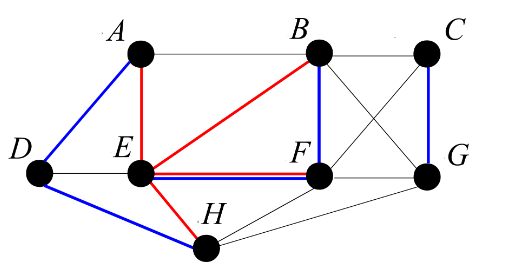
\includegraphics[width=0.6\columnwidth]{img/matroid1}
\end{center}
$$ x = \{(A, D) , (D, H) , (E , F ) , (B, F ) , (C , G )\} $$
$$ y = \{(A, E ) , (B, E ) , (E , F ) , (E , H)\} $$
$(A, D), (D, H)$ and $(C , G )$ can be added to $y$.\\

\vfill

\paragraph{TSP:} the first two axioms hold
\begin{itemize}
	\item the empty set has no sub-tours and degrees $\leq 1$
	\item any proper subset of a set $\in \mathcal{F}$ (no sub-tours and degrees $\leq 1$) also belongs to $\mathcal{F}$
\end{itemize}
but the third axiom is violated.\\
Example: $y = \{(1, 2), (2, 3)\}$ and $x = \{(3, 1), (1, 4), (4, 2)\}$.\\
No arc of $x$ can be added to $y$ remaining in $\mathcal{F}$.\\

\newpage

\subsubsection{Greedoids with the strong exchange axiom}
The optimality of the greedy algorithm can be proved for greedoids (weaker second axiom) if the exchange axiom is strengthened.\\

\textbf{Strong exchange axiom:}
$$ 
\begin{cases}
	x \in \mathcal{F}, y \in B_{\mathcal{F}} & \text{ such that } x \subset y \\
	i \in B \setminus y & \text{ such that } x \cup \left\{i\right\} \in \mathcal{F}
\end{cases}
\implies \exists j \in y \setminus x: \, 
\begin{cases}
	x \cup \left\{j\right\} \in \mathcal{F} \\
	y \cup \left\{i\right\} \setminus \left\{j\right\} \in \mathcal{F}
\end{cases}
$$

Given a basis and one of its subsets (from which the basis is accessible), if there is an element that "leads astray" the subset from the base, there must be another one which keeps it on the right way and it must be feasible to exchange the two elements in the basis.\\

Given a base $y$ and a subspace of the search space $x$, which is also a subset of the base, you can have an element $i$ not in $y$ that could be feasibly added to $x$. There must be another element inside $y$, but not $x$, that could be added to $x$ and replaced with $i$ in the base, all while remaining in the search space.\\

\paragraph{MST:} A classical example of greedoid with strong exchange axiom is given by
\begin{itemize}
	\item $B =$ edge set of a graph
	\item $\mathcal{F} =$ collection of the trees including a given vertex $v_1$
\end{itemize}
that yields Prim’s algorithm for the MST problem.\\

The trivial and the accessibility axiom hold (the heredity one does not).\\
The exchange axiom holds in the strong form.\\

\vfill

\subsubsection*{Optimal constructive algorithms}
Notice that the optimality of a constructive algorithm $A$ depends on
\begin{itemize}
	\item the \textbf{properties of the problem} (e.g., additive objective function, bases as feasible solutions)
	\item the \textbf{properties of the search space} $\mathcal{F}_A$ (that is, of the algorithm)
\end{itemize}

% End of L7

\newpage

\subsubsection{What to do when the axioms are violated}
If a search space \textbf{violates} the desired \textbf{axioms}, one can try and \textbf{change} it.\\

For the TSP, an alternative $\mathcal{F}_A$ includes all paths starting from node $1$.\\
Let $N_x$ be the set of nodes visited from $x$: the acceptable extensions are all arcs going out of the last node of path $x$ and not closing a sub-tour
$$ \Delta_A^+ (x) = \left\{(h,k) \in A : \, h = \text{ Last } (x), \, k \notin N_x \text{ or } k = 1 \text{ and } N_x = N \right\} $$

Unfortunately, the axioms are still not all satisfied
\begin{itemize}
	\item the \textbf{trivial} axiom always \textbf{holds}
	\item the \textbf{accessibility} axiom \textbf{holds}: removing the last arc yields a path starting from node $1$
	\item the \textbf{heredity} axiom does \textbf{not hold}: not all subsets are paths
	\item the \textbf{exchange} axiom does \textbf{not hold}
\end{itemize}

Therefore, it is \textbf{not even a greedoid}.\\

But the algorithm can still be a \textbf{reasonable heuristic}.\\

\newpage

\paragraph{The Nearest Neighbor heuristic for the TSP:} The Nearest Neighbor (NN) heuristic adopts the \textbf{alternative search space} keeping the \textbf{objective function} as the \textbf{selection criteria}
\begin{enumerate}
	\item \textbf{Start} with an \textbf{empty set of arcs}: $x^{(0)} = \emptyset$ that represents a degenerate path going out of node $1$ (the optimal solution certainly visits node $1$).\\
	
	\item \textbf{Find} the \textbf{arc of minimum} cost going out of the last node of $x$
	$$ (i,j) = \arg \min_{(h,k \in \Delta_A^+ (x))} c_{hk} $$
	(the objective function is additive). It's selecting the "nearest neighbor", i.e. the next closest node, without closing a sub-tour (only unseen nodes).\\
	
	\item If $j \neq 1$, go back to point $2$; otherwise, terminate ($\Delta_A^+ (x)$ allows the return to node $1$ only at the last step).\\
\end{enumerate}

The algorithm is very intuitive, and its \textbf{complexity} is $\Theta (n^2)$ ($n$ iterations, $n$ time to choose the arc of minimum cost).\\

It is not exact, but $\log n$-approximated (under the triangle inequality). You're going to find $\log n$ times the optimum, where $n$ is the number of nodes in the graph; it's not $\alpha$ approximated.\\

\newpage

\textbf{Example:} Consider a complete graph (the arcs are not reported for clarity)
\begin{center}
	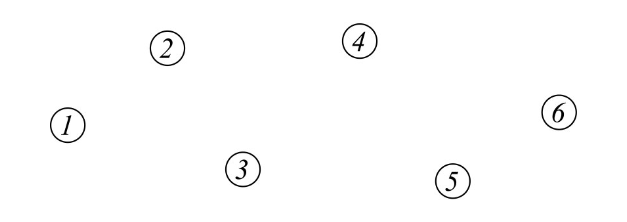
\includegraphics[width=0.5\columnwidth]{img/NNTSP1}
\end{center}
Starting from node 1 
\begin{center}
	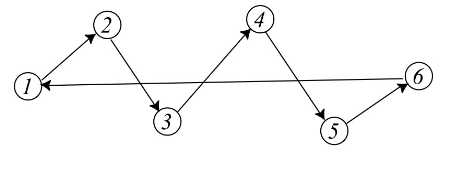
\includegraphics[width=0.5\columnwidth]{img/NNTSP2}
\end{center}
Starting from node 2
\begin{center}
	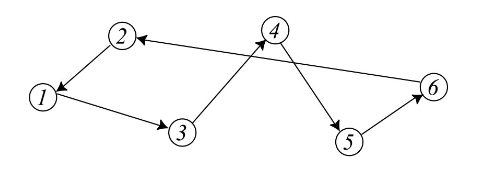
\includegraphics[width=0.5\columnwidth]{img/NNTSP3}
\end{center}
The optimal solution cannot be found starting from any node
\begin{center}
	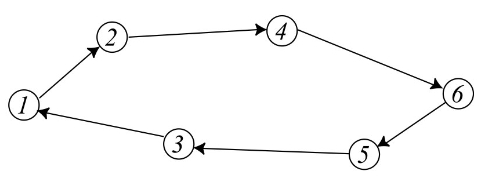
\includegraphics[width=0.5\columnwidth]{img/NNTSP4}
\end{center}

\newpage

\subsection{Heuristic constructive algorithms (HCA): the KP}
If the problem does \textbf{not admit} a \textbf{search space} with \textbf{suitable properties}, one must keep into account the \textbf{constraints of the problem} adopting
\begin{enumerate}
	\item not only a \textbf{good definition} of $\mathcal{F}_A$
	\item but also a \textbf{sophisticated definition of the selection criteria} $\varphi_A (i, x)$
\end{enumerate}
This allows effective results, even if not provably optimal.\\

In the KP, the drawback derives from the volume of the objects: promising objects have a large value, but also a small volume
\begin{itemize}
	\item define the \textbf{selection criteria} as the unitary value $\varphi_A (i, x) = \phi_i / v_i$ (getting the "value" of each piece to determine which is best)
\end{itemize}

The resulting algorithm
\begin{itemize}
	\item can perform very badly
	\item with a small modification is 2-approximated
\end{itemize}

\vfill

\paragraph{Example:}
\begin{center}
	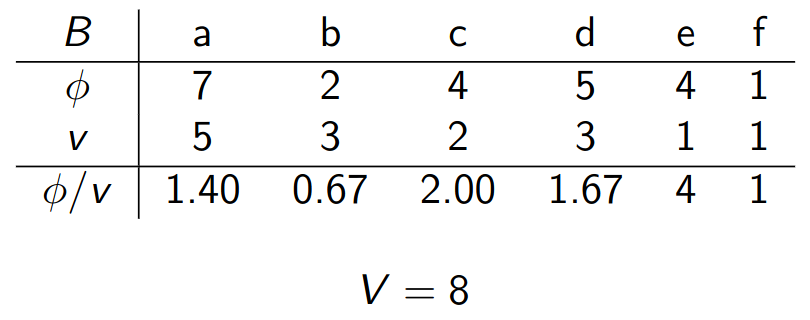
\includegraphics[width=0.5\columnwidth]{img/HKP1}
\end{center}
The algorithm performs the \textbf{following steps}:
\begin{enumerate}
	\item $x := \emptyset$
	\item select $i := e$ and update $x := \{e\}$
	\item select $i := c$ and update $x := \{c, e\}$
	\item select $i := d$ and update $x := \{c, d, e\}$
	\item select $i := f$ and update $x := \{c, d, e, f \}$ (object $a$ does not fit)
	\item since $\Delta_A^+ (x) = \emptyset$, terminate
\end{enumerate}
The value of the solution found is $14$, the optimal solution is $x^\ast = \{a, c, e\}$ and its value is $15$. There can be critical cases with indefinitely bad gaps (it can discard large objects, even if they have large value).

\newpage

\subsubsection{2-Approximated algorithm for the KP}
Steps
\begin{enumerate}
	\item \textbf{Start} with an \textbf{empty subset}: $x^{(0)} = \emptyset$
	
	\item Find the \textbf{object} $i^{(t)}$ of \textbf{maximum unitary value} in $B \setminus x^{(t−1)}$:
	$$ i^{(t)} := \arg \max_{i \in B \setminus x^{(t-1)}} \frac{\phi_{i^{(t)}}}{v_{i^{(t)}}}$$
	it considers all elements, not only the one that respect the capacity.\\
	
	\item If it respects the capacity, \textbf{add} $i^{(t)}$ to $x^{(t−1)}$: $x^{(t)} := x^{(t−1)} \cup \{i^{(t)}\}$ and go \textbf{back to} point $2$.\\
	
	\item Build a \textbf{solution} with the \textbf{first rejected object}: $x' = \{i^{(t)}\}$.\\
	
	\item \textbf{Return the better solution} between $x$ and $x'$: $f_A = \max \left[f (x), f (x')\right]$.\\
\end{enumerate}


It is easy to prove that
\begin{itemize}
	\item \textbf{the sum of the two solution values overestimates the optimum}
	$$ f(x) + f(x') = \sum_{\tau = 1}^{t} \phi_{i^{(\tau)}} \geq f^\ast $$
	This sum essentially represents a solution for a "bigger knapsack" (it exceeds the capacity), so it will obviously be better (upper bound).\\
	
	\item \textbf{the best of the two solution values is at least half their sum}
	$$ f_A = \max \left[ f(x), f(x')\right] \geq \frac{f(x) + f(x')}{2} \geq \frac{1}{2} f^\ast$$
	The larger one will obviously be more than half our earlier sum, which is larger than the optimal solution $\implies$ it will be larger than half the optimal solution.\\
\end{itemize}

\newpage

\subsection{Pure and adaptive constructive algorithms}
A constructive algorithm $A$ is
\begin{itemize}
	\item \textbf{Pure} if the selection criteria $\varphi_A$ depends only on the new element $i$. The decision is made only on what to add, independently of the "past choices".\\
	
	\item \textbf{Adaptive} if $\varphi_A$ depends both on $i$ and on the current solution $x$.\\
\end{itemize}

Many criteria $\varphi_A (i, x)$ admit \textbf{equivalent forms} depending only on $i$
\begin{itemize}
	\item In the TSP, $\varphi_A ((i, j), x) = f (x \cup \{(i, j)\})$ is equivalent to $c_{ij}$.\\
	
	\item In the KP, $\varphi_A (i, x) = f (x \cup \{i\})$ is equivalent to $\phi_i$
\end{itemize}

So far, we have seen only pure constructive algorithms.\\

An \textbf{additive selection criteria} yields a \textbf{pure constructive algorithm}.\\

\newpage

\subsection{HCA: Set Covering}
Given a binary matrix and a cost vector associated to the columns, find a minimum cost subset of columns covering all the rows (at least one $1$ for each row, choose columns, minimum cost).\\

The \textbf{objective} is \textbf{additive}, but the solutions are \textbf{not maximal subsets} (actually, the smaller feasible subsets are better).\\

An \textbf{adaptive selection criteria} $\varphi_A (i, x)$ is necessary: a pure one ($\varphi_A (i)$) could repeatedly choose columns covering the same rows.\\

The more promising \textbf{ideas} are to consider
\begin{itemize}
	\item the \textbf{objective function}: select columns of low cost
	\item the \textbf{constraints}: select columns covering many rows
	\item the \textbf{current subset} $x$: select columns covering new rows
\end{itemize}

In \textbf{summary}
\begin{itemize}
	\item include in $\Delta_A^+ (x)$ only \textbf{columns covering additional rows} not in $x$
	\item apply the \textbf{adaptive selection criteria} $\varphi_A (i, x) = c_i / a_i (x)$ where $a_i (x)$ is the number of rows covered by $i$, but not by $x$. 
\end{itemize}

In the calculation we must take into account the columns we already covered, the selection criteria must consider only columns that have yet to be covered. This means that the algorithm must be adaptive, it can't be pure, otherwise it would choose "useless" columns.\\
This is taken into account inside the definition of $a_i (x)$, which is defined as the number of rows covered by $i$, but not by $x$. \\

\newpage

\paragraph{Example:} this algorithm has the optimum as an upper bound, but it can also fail
$$
c \;\;\;\;
\begin{array}{| c c c c c |}
	\hline
	25 & 6 & 8 & 24 & 12 \\
	\hline
\end{array}
$$

$$
A \;\;\;\;
\begin{array}{| c c c c c |}
	\hline
	1 & 1 & 0 & 0 & 0 \\
	1 & 1 & 0 & 0 & 0 \\
	1 & 1 & 1 & 0 & 0 \\
	1 & 0 & 1 & 1 & 0 \\
	1 & 0 & 0 & 1 & 0 \\
	1 & 0 & 0 & 0 & 1 \\
	\hline
\end{array}
$$
The algorithm performs the following \textbf{steps}:
\begin{itemize}
	\item $x := \emptyset$
	\item since $c/a_i (x) = [4.1\overline{6}, \; 2, \; 4, \; 12, \; 12 ]$, select $i := 2$
	\item since $c/a_i (x) = [8.\overline{3}, \; -, \; 8, \; 12, \; 12 ],$ select $i := 3$
	\item since $c/a_i (x) = [12.5, \; -, \; -, \; 24, \; 12 ]$, select $i := 5$
	\item since $c/a_i (x) = [25, \; -, \; -, \; 24, \; - ]$, select $i := 4$
	\item all the rows are covered, therefore $\Delta_A^+ (x) = \emptyset$ and terminate
\end{itemize}
The solution returned is $x = \{2, 3, 4, 5\}$ and its value is 50, whereas the optimal solution $x^\ast = \{1\}$ has value $f^\ast = 25$.\\

\newpage

\subsubsection{Approximability of the SCP}
This algorithm has a \textbf{non-constant} (logarithmic) \textbf{approximation ratio}
\begin{itemize}
	\item At each step $t$, each column $i$ is evaluated with \textbf{criteria}
	$$ \varphi_A \left(i, x^{(t-1)}\right) = \frac{c_i}{a_i \left(x^{(t-1)}\right)} $$
	estimate of the unitary cost, cost of a column divided by the number of covered rows that are not already covered by the current solution.\\
	
	\item \textbf{Row} $j$ is \textbf{covered} by a certain \textbf{column} ($i_j$) at a certain \textbf{step} ($t_j$).\\
	
	\item Start assigning \textbf{weight} $\theta_j = 0$ to each \textbf{row} $j$.\\
	
	\item When each \textbf{row} $j$ is \textbf{covered} (step $t_j$), set its \textbf{weight} to
	$$ \theta_j = \frac{c_{i_j}}{a_{i_j} \left(x^{(t_j - 1)}\right)}$$
	so that the total weight of the rows increases by $c_{i_j}$ at step $t_j$; correspondingly, $x$ includes column $i_j$ and its cost increases by $c_{i_j}$.\\
	When you choose a column, put it in the partial solution and increase the cost of the solution by $c_{i_j}$, now modify the weights of the rows, take the cost of the column $c_{i_j}$ and divide it by how many new rows are covered, give each of these rows this increase in weight.\\
	
	\item The \textbf{total cost} of $x$ is always equal to the \textbf{total weight of the rows}
	$$ f_A (x) = \sum_{i \in x} c_i = \sum_{j \in R} \theta_j $$
	\nn
	
	\item at \textbf{step} $t$, there are $|R^{(t)}| \leq |R| − t$ \textbf{uncovered rows}.\\
	
	\newpage
	
	\item the columns of the optimal solution could cover them all with \textbf{cost} $f^\ast \implies$ at least one of such columns has \textbf{unitary cost} $\leq f^\ast /|R^{(t)}|$.\\
	
	\item the column $i$ selected has \textbf{minimum unitary cost} $\varphi_A (i, x^{(t−1)})$, therefore $\leq f^\ast /|R^{(t)}|$ and the covered rows \textbf{increase their weight} by
	$$ \theta_j = \varphi_A (i, x^{(t-1)}) \leq \frac{f^\ast}{|R^{(t_j)}|} \implies \sum_{j \in R} \theta_j \leq \sum_{j \in R} \frac{f^\ast}{|R^{(t_j)}|} $$
	The cost to cover each row $j$ is not larger than the optimum divided by the number of rows uncovered at the step in which $j$ gets covered.\\
	
	\item the integer number $|R^{(t)}|$ strictly \textbf{decreases} at each step.\\
	
	\item the sum can be \textbf{overestimated reducing} $|R^{(t)}|$ by $1$ at each step.\\
	
	\item The \textbf{approximation ratio} is limited by a \textbf{logarithmic guarantee}
	$$ f_A = \sum_{j \in R} \theta_j \leq \sum_{j \in R} \frac{f^\ast}{|R^{(t_j)}|} \leq \sum_{r=|R|}^1 \frac{f^\ast}{r} \leq \left(\ln |R| + 1\right) f^\ast $$
\end{itemize}

\newpage

\subsection{HCA: Bin Packing Problem}
Another adaptive problem, the BPP requires to divide a set $O$ of voluminous objects into the minimum number of containers of given capacity drawn from a set $C$.\\

$B = O \times C$ includes the \textbf{object-container assignments} $(i, j)$
\begin{itemize}
	\item with exactly \textbf{one container for each object}
	\item with the \textbf{total volume} in each container \textbf{not exceeding} the \textbf{capacity}
\end{itemize}

Let us define the \textbf{search space} $\mathcal{F}_A$ as the set of \textbf{all partial solutions}.\\

The \textbf{objective function} is a \textbf{bad selection criteria}, because it is flat.\\
All the augmented subsets have the same value or increase it by $1$.\\

\subsubsection{First-Fit heuristic}
Consider the \textbf{object-container pairs} lexicographically
\begin{itemize}
	\item \textbf{Start} with an \textbf{empty subset}: $x^{(0)} = \emptyset$
	\item \textbf{Select pair} $(i, j)$ according to the following criteria:
	\begin{itemize}
		\item $i$ is the \textbf{first} (minimum index) \textbf{unassigned object}
		\item $j$ is the \textbf{first container with enough residual capacity} for $i$ (a used container, if possible; an unused one otherwise)
	\end{itemize}
	\item \textbf{Add} the new \textbf{assignment} to the \textbf{solution}: $x^{(t)} := x^{(t−1)} \cup \{(i, j)\}$
\end{itemize}

Notice that the \textbf{choice} of $(i, j)$
\begin{itemize}
	\item \textbf{does not minimize} $f (x \cup \{(i, j)\})$ (another $i$ could be better)
	\item is split into \textbf{two phases} (first $i$, then $j$)
\end{itemize}

Essentially, take each element and put it into the first container you find with enough space, used or otherwise.\\

\newpage

\paragraph{Example:}
\begin{center}
	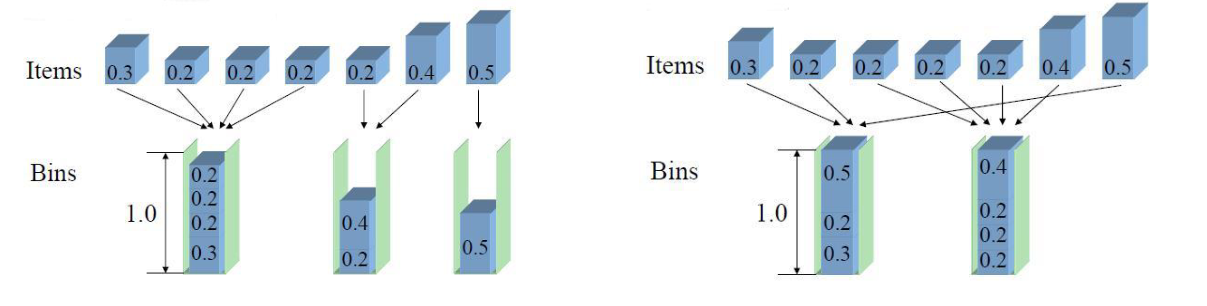
\includegraphics[width=\columnwidth]{img/CHBPP1}
\end{center}
\textbf{The solution is not optimal}; but it is \textbf{approximated}:
\begin{itemize}
	\item At least $f^\ast \geq \sum_{i \in O} v_i / V$ \textbf{containers} are \textbf{necessary}. Lower bound, the minimum number of container if you could completely fill them all, it must be $\leq$ than the optimal solution.\\
	
	\item The \textbf{occupied volume} is $> V/2$ for \textbf{all used containers}, possibly except for the last one (if a second half-empty container existed, its objects would have been assigned to the first, it would be a contradiction).\\
	
	\item The \textbf{total volume exceeds} that of the $f_A − 1$ "saturated" containers
	$$ \sum_{i \in O} v_i > (f_A - 1)\frac{V}{2} $$
	This means that the total volume is more than $f_A - 1$ (if the last is not more than half full) times $V/2$ (lower bound).\\
	Which implies $(fA − 1) < 2/V \sum_{i \in O} v_i \leq 2f^\ast \implies f_A \leq 2f^\ast$. Our solution is less than the volume of the "saturated" containers expressed before, which in turn is smaller than the optimal solution, refactor the equation and we get the last part, our solution is less than twice the optimum $+1$.\\
	The analysis can be improved to 1.7.\\
\end{itemize}

\newpage

\paragraph{Better choices?} The \textbf{approximation ratio} $\alpha = 2$ holds for \textbf{any permutation} of the objects.\\

Intuition would suggest selecting first the smallest objects, in order to keep the objective $f (x \cup \{i\})$ as small as possible, but this neglects that all objects must be assigned.\\

By contrast, it is \textbf{better to select the largest object first} because
\begin{itemize}
	\item each object in a container has a volume strictly larger than the residual capacity of all the previous containers (otherwise, it would have been assigned to one of them)
	\item keeping the smallest objects in the end guarantees that many containers have a small residual capacity
\end{itemize}
This algorithm has a \textbf{better approximation ratio}: $f_A \leq (11/9) f^\ast + 1$.\\

The difference is that instead of choosing the object of minimum index you choose the object of largest volume.\\

% End of L8

\newpage

\subsection{Extensions of the basic constructive scheme}
The \textbf{basic scheme} of constructive algorithms can be \textbf{enhanced} using
\begin{enumerate}
	\item a \textbf{more effective construction graph}
	\begin{itemize}
		\item \textbf{add more than one element} to the current subset $x$
		\item add elements to $x$, but \textbf{also remove elements} from $x$ (without going back to visited subsets, otherwise the construction graph would be cyclic)
	\end{itemize}
	\nn
	
	\item a \textbf{more sophisticated selection criteria}, such as
	\begin{itemize}
		\item a \textbf{regret-based function} that estimates potential future losses associated with element $i$
		\item a \textbf{look-ahead function} that estimates the final value of the objective obtained adding $i$ to $x$
	\end{itemize}
\end{enumerate}

\newpage

\subsubsection{Extensions of the construction graph}
The constructive algorithm adds an element at a time to the solution.\\

It is possible to \textbf{generalize} this scheme with algorithms that at each step
\begin{enumerate}
	\item \textbf{Add more than one element:} the selection criteria $\varphi_A (B^+, x)$ identifies a subset $B^+ \subseteq B \setminus x$ to add, instead of a single element $i$. \\
	The criteria depends not only from $x$ but also on the subset of the ground set $B^+$.\\
	
	\item Add elements, but also \textbf{remove a smaller number of elements:} the selection criteria $\varphi_A (B^+, B^-, x)$ identifies a subset $B^+ \subseteq B \setminus x$ to add and a subset $B^- \subseteq x$ to remove, with $|B+| > |B-|$. \\
	The criteria becomes a function of $x$, $B^+$ and the subsets of element currently included in $x$ to remove $B^-$.\\
\end{enumerate}

These algorithms build an \textbf{acyclic construction graph} on the search space, so that they never revisit any subset.\\

The fundamental problem is to \textbf{define a family} $\Delta_A^+ (x)$ of subset pairs such that \textbf{optimizing the selection criteria is a polynomial problem}
$$ \min_{(B^+, B^-) \in \Delta_A^+ (x)} \varphi_A (B^+, B^-, x) $$
that is
\begin{itemize}
	\item subsets \textbf{efficiently optimizable} (minimum paths, \dots)
	\item subsets of \textbf{limited size} (e.g., $|B^+| = 2$ and $|B^-| = 1$)
\end{itemize}

Minimizing the selection criteria can become difficult, there could be exponentially many subsets. To counteract that we can limit the size of our subsets $B^+$ and $B^-$ or define specific families for these subsets such that they are "classic problems" and consequently easily optimizable (e.g. minimum paths).\\

\newpage

\subsection{The Steiner Tree Problem (STP)}
Given an undirected graph $G = (V , E )$, a cost function $c : E \rightarrow \mathbb{N}$ on the edges and a subset of special vertices $U \subset V$, find a tree connecting at minimum cost all special vertices.
\begin{center}
	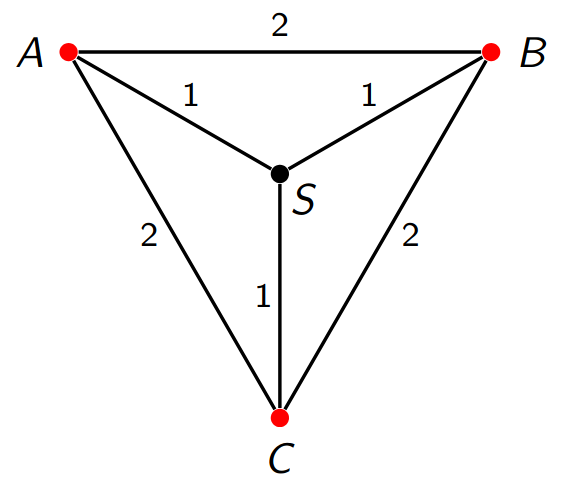
\includegraphics[width=0.6\columnwidth]{img/STP1}
\end{center}
The minimum tree spanning the special vertices is not necessarily optimal (and it might not even exist).\\

Basically, connect the special dots and make it quick.\\

\newpage

\subsubsection{Distance Heuristic (DH) for the STP}
A basic constructive algorithm could adopt the same \textbf{search spaces} as
\begin{itemize}
	\item Kruskal's algorithm: the set of \textbf{all forests}
	\item Prim's algorithm: the set of \textbf{all trees including a (special) vertex}
\end{itemize}

but adding \textbf{one edge at a time}
\begin{itemize}
	\item returns solutions with \textbf{redundant edges}, therefore expensive
	\item has a hard time \textbf{distinguishing useful and redundant} edges
\end{itemize}

The Distance Heuristic adopts as \textbf{search space} $\mathcal{F}$ the \textbf{collection of all trees including a given special vertex} $v_1$ (as in Prim).\\

It iteratively \textbf{adds a path} $B^+$ \textbf{between} $x$ \textbf{and a special vertex} instead of a single edge, so that
\begin{itemize}
	\item $x$ \textbf{remains a tree}
	\item $x$ \textbf{spans a new special vertex}
	\item the \textbf{minimum cost path} can be \textbf{computed efficiently} at each step
\end{itemize}

It \textbf{terminates} when \textbf{all special vertices are connected}.\\

Instead of adding only one edge at a time, at each step it adds the minimum cost path from an already visited vertex (not necessarily special) to the next closest special vertex, keeping the solution less redundant and simplifying the computation of the minimum cost path.\\

\newpage

\paragraph{Example:}
\begin{center}
	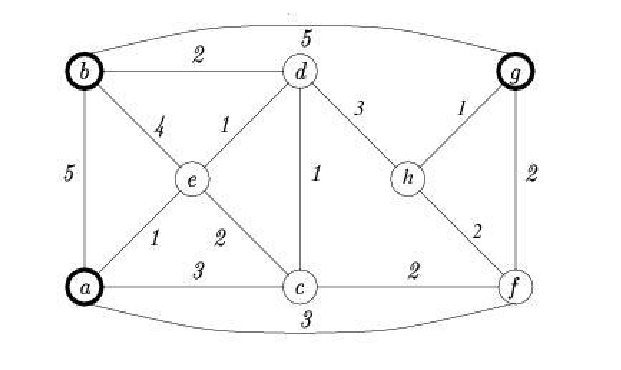
\includegraphics[width=0.7\columnwidth]{img/STP2}
\end{center}

\begin{itemize}
	\item Start with a single special vertex $a$: $x := \emptyset$ (degenerate tree).\\
	
	\item Add the closest special vertex ($b$) through path $(a, e, d, b)$:
	$$ x = \{(a, e) , (e, d) , (d, b)\} $$
	
	\item Add the closest special vertex ($g$) through path $(g , h, d)$:
	$$ x = \{(a, e) , (e, d) , (d, b) , (g , h) , (h, d)\} $$
	The Distance Heuristic algorithm is 2-approximated: it is equivalent to computing a minimum spanning tree on a graph with
	\begin{itemize}
		\item vertices reduced to the special vertices
		\item edges corresponding to the minimum paths
	\end{itemize}
	You can think of it as a graph with only special vertices and the minimum path between them as edges.\\
	
	\item All special vertices are in the solution: terminate (this time the solution is optimal)
\end{itemize}

\newpage

\paragraph{Counterexample to optimality:} Consider a complete graph $G = (V , E )$ with $U = V \setminus \{1\}$ and cost
$$ 
c_{uv} = \begin{cases}
	(1 + \epsilon)M & \text{ for } u \text{ or } v = 1 \\
	2M & \text{ for } u,v \in U
\end{cases}
$$
($M$ is just used to obtain integer costs for any $\epsilon$).\\
Every arc from node 1 cost $(1 + \epsilon)M$, $2M$ for everything else.\\

The DH returns a star spanning the special vertices: $f_{DH} = (n − 2) \cdot 2M$.\\

The optimal solution is a spanning star centered in $1$: $f^\ast = (n − 1) \cdot (1 + \epsilon)M$.

\begin{center}
	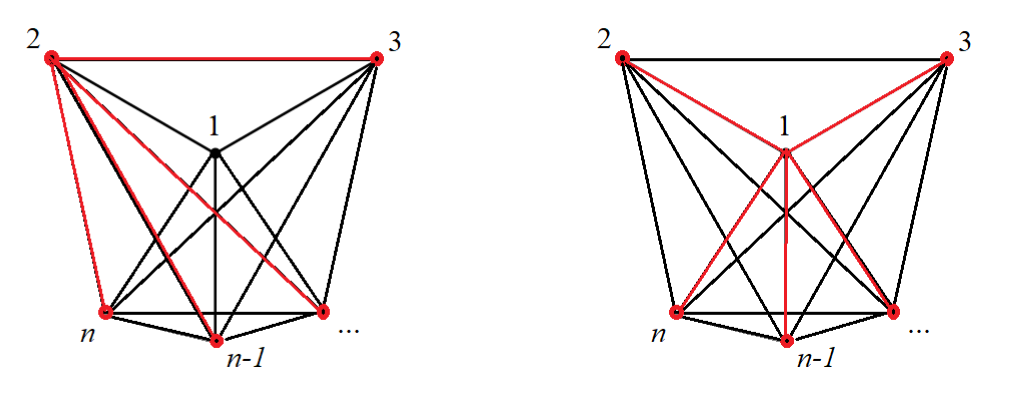
\includegraphics[width=0.9\columnwidth]{img/STP3}
\end{center}

The approximation ratio is 
$$ \rho_{DH} = \frac{f_{DH}}{f^\ast} = \frac{n-2}{n-1} \cdot \frac{2}{1 + \epsilon} < 2 $$
and converges to $2$ as $n$ increases and $\epsilon$ decreases.\\

\newpage

\subsection{Insertion algorithms for the TSP}
Several heuristic algorithms for the TSP define the \textbf{search space} $\mathcal{F}_A$ as the \textbf{set of all circuits} of the graph \textbf{including a given node}; a circuit
\begin{itemize}
	\item \textbf{cannot} be obtained from another one by \textbf{adding a single arc}
	\item \textbf{can} be obtained \textbf{adding two arcs} $(i, k)$, $(k, j)$ and \textbf{removing one} $(i, j)$
\end{itemize}

\begin{center}
	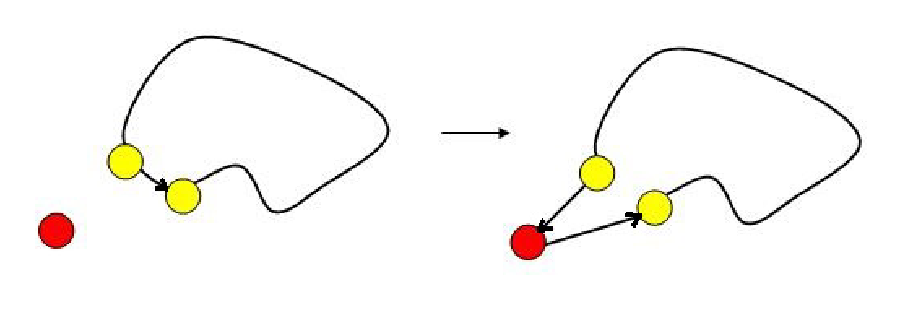
\includegraphics[width=0.8\columnwidth]{img/IATSP1}
\end{center}

Steps
\begin{enumerate}
	\item Start with a \textbf{zero-cost self-loop on node} $1$: $x^{(0)} = \{(1, 1)\}$ (Not much different from an \textbf{empty set})
	
	\item Select a \textbf{node} $k$ to be \textbf{added} and an \textbf{arc} $(i, j)$ to be \textbf{removed}
	
	\item If the circuit \textbf{does not visit all nodes}, go back to point $2$; \textbf{otherwise terminate}
\end{enumerate}

Such a scheme \textbf{never visits again the same solution} and builds a \textbf{feasible solution in} $n - 1$ steps (each step adds a new node).\\

Start from a circuit, add one node at a time by adding a new edge and removing an old one.\\

\newpage

\subsubsection{Cheapest Insertion heuristic} 
The selection criteria $\varphi_A (B^+, B^-, x)$ must \textbf{choose an arc and a node}; there are $(n − |x|) |x| \in O (n^2)$ alternatives
\begin{itemize}
	\item $|x|$ possible \textbf{arcs} ($s_i , s_{i+1}$) to \textbf{remove}; the nodes already in the circuit
	\item $n − |x|$ possible \textbf{nodes} $k$ to \textbf{add} through the arcs ($s_i , k$) and ($k, s_{i+1}$); nodes not yet in the circuit that can be added
\end{itemize}

The \textbf{Cheapest Insertion} (CI) heuristic uses as a \textbf{selection criteria}
$$ \varphi_A (B^+, B^-, x) = f \left(x \cup B^+ \setminus B^- \right) $$

\textbf{Objective function} $f (x)$ is \textbf{additive}, hence \textbf{extensible} to the whole of $\mathcal{F}_A$.\\

Here $k$ denotes a general node outside the circuit, $s_i$ (or anything $s$-related) denotes nodes already inside the circuit.\\

Since $f (x \cup B^+ \setminus B^-) = f (x) + c_{s_i ,k} + c_{k,s_{i+1}} - c_{s_i ,s_{i+1}}$ (objective function $+$ the cost of the arcs added $-$ the cost of the arc removed)
$$ \arg \min_{B^+, B^-} \varphi_A \left(B^+, B^-, x \right) = \arg \min_{i,k} (c_{s_i, k} + c_{k, s_{i+1}} - c_{s_i, s_{i+1}})$$
We need to minimize these terms by choosing the set of $i,k$ that minimizes the variation in cost. \\

The \textbf{computational cost of evaluating} $\varphi_A$ \textbf{decreases} from $\Theta (n)$ to $\Theta (1)$ (since we need to compute only the variation).\\

\newpage

\paragraph{Algorithm Cheapest Insertion:}
\begin{enumerate}
	\item Start with a \textbf{zero-cost self-loop} on node $1$: $x^{(0)} = \{(1, 1)\}$. It is also like starting with a single node.
	
	\item Select the \textbf{arc} $(s_i , s_{i+1}) \in x$ and the \textbf{node} $k \notin N_x$ \textbf{such that} ($c_{s_i, k} + c_{k, s_{i+1}} − c_{s_i ,s_{i+1}}$) is minimum; select the node to add and the arc to remove, such that the total variation is at a minimum.
	
	\item If the circuit does not visit all nodes, go back to point $2$; otherwise terminate.
\end{enumerate}
It is not exact, but \textbf{2-approximated}, under the triangle inequality.\\

The CI algorithm performs $n - 1$ steps: at each step $t$
\begin{itemize}
	\item it evaluates $(n - t) t$ node-arc pairs
	\begin{itemize}
		\item each evaluation requires constant time
		\item each evaluation possibly updates the best move
	\end{itemize}
	\item it performs the best addition/removal
	\item it decides whether to terminate
\end{itemize}

The \textbf{overall complexity} is $\Theta (n^3)$.\\

It can be reduced to $\Theta (n^2 \log n)$ collecting in a min-heap the insertion costs for each external node: each of the $n$ steps
\begin{itemize}
	\item selects the best insertion in $O (n)$ time and performs it
	\item creates two new insertions and removes one for each external node, and updates their heaps in $O (n \log n)$ time
\end{itemize}

\newpage

\subsubsection{Nearest Insertion heuristic}
The algorithm Cheapest Insertion tends to select nodes close to circuit $x$: minimizing $c_{s_i ,k} + c_{k,s_{i+1}} - c_{s_i ,s_{i+1}}$ implies that $c_{s_i ,k}$ and $c_{s_{i+1},k}$ are small (looks for the closest node to add, the weight of the arcs to that node must be small).\\

To accelerate, one can \textbf{decompose criteria} $\varphi_A$ \textbf{into two phases}.\\

\paragraph{Algorithm Nearest Insertion (NI):}
\begin{enumerate}
	\item start with a \textbf{zero-cost self-loop} on node $1$: $x^{(0)} = \{(1, 1)\}$
	
	\item \textbf{Add criteria:} select the \textbf{node} $k$ \textbf{nearest to circuit} $x$
	$$ k = \arg \min_{l \notin N_x} \left(\min_{s_i \in N_x} c_{s_i, l} \right) $$
	It chooses the minimum distance among the minimum distances of each node from the circuit.
	
	\item \textbf{Delete criteria:} select the \textbf{arc} ($s_i , s_{i+1}$) that \textbf{minimizes} $f$
	$$ (s_i, s_{i+1}) = \arg \min_{s_i, s_{i+1} \in x} \left(c_{s_i, k} + c_{k, s_{i+1}} - c_{s_i, s_{i+1}}\right) $$
	The arc to break is the one that minimizes the objective function.
	
	\item If the circuit does not visit all nodes, go back to point 2; otherwise terminate
\end{enumerate}

It is not exact, but \textbf{2-approximated}, under the triangle inequality.\\

Instead of choosing together node and arc, you first choose the node and, given the node, the arc is chosen; you look for the node closest to the circuit in general. \\
Instead of minimizing the new cost, the cost of the arc that connects the new node to the circuit is minimized.\\

\newpage

The NI algorithm performs $n - 1$ steps: at each step $t$ it
\begin{itemize}
	\item \textbf{Evaluates the distance} of $(n - t)$ nodes from the circuit (the remaining nodes), each one in $\Theta (t)$ time (confront them with the nodes already in the circuit); it makes this $\Theta (n^2)$.\\
	
	\item \textbf{Selects} the \textbf{node at minimum distance}.\\
	
	\item \textbf{Evaluates the removal} of $t$ arcs, each one in $\Theta (1)$ time.\\
	
	\item Performs the \textbf{best addition/removal}.\\
	
	\item \textbf{Decides} whether to \textbf{terminate}.\\
\end{itemize}

The \textbf{overall complexity} is $\Theta (n^3)$.\\

It \textbf{can be reduced to} $\Theta (n^2)$ collecting in a vector for each external node the closest internal node: each of the $n - 1$ steps
\begin{itemize}
	\item selects the closest node in $O (n)$ time
	\item finds the insertion point in $O (n)$ time
	\item inserts the node creating a new internal node for each external node, which possibly becomes the closest saved in the vector; each of the $O (n)$ updates takes $O (1)$ time
\end{itemize}

It has the same approximation guarantee as the last heuristic, but it's faster.\\

\newpage

\subsubsection{Farthest Insertion heuristic}
The choice of the closest node to the cycle is natural, but misleading: since all nodes must be visited, it is preferable to service in the best way the most problematic ones (i.e., the farthest ones).\\

\paragraph{Algorithm Farthest Insertion (FI):}
\begin{enumerate}
	\item Start with a \textbf{zero-cost self-loop} on node $1$: $x^{(0)} = \{(1, 1)\}$.\\
	
	\item \textbf{Add criteria:} select the node $k$ \textbf{farthest} from cycle $x$
	$$ k = \arg \max_{l \notin N_x} \left(\min_{s_i \in N_x} c_{s_i, l}\right) $$
	(the node that is farthest from the closest node of the cycle) the maximum of the minimum distances from the circuit.\\
	
	\item \textbf{Delete criteria:} select the arc ($s_i , s_{i+1}$) minimizing
	$$ (s_i, s_{i+1}) = \arg \min_{(s_i, s_{i+1} \in x} \left(c_{s_i, k} + c_{k, s_{i+1}} - c_{s_i, s_{i+1}} \right) $$
	
	\item If the circuit does not visit all nodes, go back to point 2; otherwise terminate.\\
\end{enumerate}

It is \textbf{$\log n$-approximated} under the triangle inequality, hence \textbf{worse} than the previous ones in the \textbf{worst-case} (but often \textbf{experimentally better}).\\

\newpage

It starts by inserting the furthest possible nodes (but includes them in the best way), until it forms a complete circuit. This way the "isolated" nodes can be connected first and penalize less the final result.\\

The FI algorithm performs $n - 1$ steps: at each step $t$
\begin{itemize}
	\item it \textbf{evaluates the distance} of $(n - t)$ nodes from the circuit, each one in $\Theta (t)$ time
	\item \textbf{select} the node at \textbf{maximum distance}
	\item it \textbf{evaluates the removal} of $t$ arcs, each one in $\Theta (1)$ time
	\item it performs the \textbf{best addition/removal}
	\item it \textbf{decides} whether to \textbf{terminate}
\end{itemize}

The complexity is the same as the NI (just with the farthest).\\

The overall complexity is $\Theta (n^3)$.\\

It can be reduced to $\Theta (n^2)$ as in the NI heuristic.\\

\newpage

\subsection{Regret-based constructive heuristics}
We've seen how to make a more effective construction graph, the other method to extend a constructive algorithm is a more sophisticated selection criteria, such as a look-ahead or regret-based function.\\

\textbf{Decisions taken in early steps can severely restrict the feasible choices} in later steps due to the \textbf{constraints} of the problem
\begin{itemize}
	\item \textbf{BPP:} all objects must be put into a container, but early assignments could make some containers unavailable for later objects
	
	\item \textbf{TSP:} all nodes must be visited, but early routing decisions could make the visit of later nodes more expensive (even impossible, if the graph is noncomplete)
	
	\item \textbf{CMST:} all vertices must be linked to the root through a subtree, but early links could make some subtrees unavailable for later vertices
\end{itemize}

The selection criteria can take it into account \textbf{implicitly}
\begin{itemize}
	\item \textbf{BPP:} the Decreasing First-Fit heuristic assigns the larger objects first
	\item \textbf{TSP:} the Farthest Insertion heuristic visits the farther nodes first
\end{itemize}

Some selection criteria aim explicitly to \textbf{leave larger sets of good choices}.\\

\paragraph{Regret criteria:} A typical regret-based heuristic consists in
\begin{itemize}
	\item \textbf{partitioning} $\Delta_A^+ (x)$ into disjoint classes of choices (the assignments of each object, how every object can be assigned, the edges incident in each vertex)
	
	\item compute a \textbf{basic selection criteria} for all choices
	
	\item compute \textbf{for each class the regret}, i.e. the \textbf{difference} between either
	\begin{itemize}
		\item the \textbf{second-best choice} or
		\item the \textbf{average of the other choices} (possibly weighted)
	\end{itemize}
	and the best choice in order to estimate the damage incurred by postponing the best choice until it becomes impossible
	
	\item \textbf{choose} the \textbf{best choice} of the class for which the \textbf{regret is maximum}. This is effective when a single choice per class must be taken
\end{itemize}

Essentially we divide the possible additions into classes (for example all the feasible assignments of an object is a single class), and pick the (greedy) best choice for each class. To choose from which class to pick the best choice, we use the regret, maximizing it.\\

The regret represents how much worse the other choices will be, so we choose the best choice of the class with the highest regret, "fearing" that if we don't pick that option now, we'll be forced to pick a much worse one later on. \\

You can make this reasoning when you're sure that you will have to take at least one choice for each class.\\

\paragraph{Example:} Consider the CMSTP and ground set $B = V \times T$ ($(vertex,subtree)$ pairs). Let the weights be uniform ($w_v = 1$ for all $v \in V$) and capacity $W = 2$

\begin{center}
	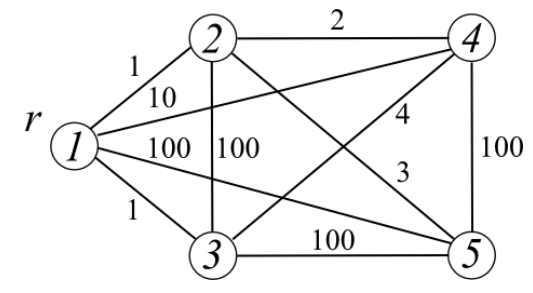
\includegraphics[width=0.5\columnwidth]{img/RBCSMTP}
\end{center}

Let the search space $\mathcal{F}$ include all partial solutions.\\

The greedy algorithm puts vertex $2$ in subtree $1$, vertex $3$ in subtree $2$; then vertex $4$ in subtree $1$ and finally vertex $5$ in subtree $3$:
$$ c(x) = 1 + 1 + 2 + 100 = 104$$ 

The regret algorithm puts vertex $2$ in subtree $1$, vertex $3$ in subtree $2$; now:
\begin{itemize}
	\item the regret of vertex $3$ is the difference $c(3, 3) − c(3, 2) = 1 − 1 = 0$
	\item the regret of vertex $4$ is the difference $c(4, 2) − c(4, 1) = 10 − 2 = 8$
	\item the regret of vertex $5$ is the difference $c(5, 2) − c(5, 1) = 100 − 3 = 97$
\end{itemize}
The algorithm puts vertex $5$ in subtree $1$.\\
Then, it proceeds putting vertices $2$ and $4$ in subtree $2$:
$$ c(x) = 1 + 3 + 1 + 4 = 9 $$

\newpage

\subsection{Roll-out heuristics}
They are also known as \textbf{single-step look-ahead constructive heuristics} and were proposed by Bertsekas and Tsitsiklis (1997).\\

Given a \textbf{basic constructive heuristic} $A$
\begin{itemize}
	\item \textbf{start} with an \textbf{empty subset}: $x^{(0)} = \emptyset$
	
	\item at each step $t$
	\begin{itemize}
		\item \textbf{extend} the \textbf{subset} in \textbf{each feasible way}: $x^{(t−1)} \cup \{i\}$, $\forall i \in \Delta_A^+ (x)$
		
		\item \textbf{apply} the \textbf{basic heuristic} to \textbf{each extended subset} and compute the resulting solution $x_A (x^{(t−1)} \cup \{i\})$
		
		\item use the \textbf{value of the solution} as the \textbf{selection criteria} to choose $i^(t)$
		$$ \varphi_A (i,x) = f \left(x_A \left(x^{(t-1)} \cup \left\{i\right\} \right) \right)$$
	\end{itemize}
	
	\item \textbf{terminate} when $\Delta_A^+ (x)$ is empty
\end{itemize}

Try every feasible move, look at the result, go back and choose the move. \\

The \textbf{result} of the roll-out heuristic \textbf{dominates that of the basic heuristic} (under very general conditions). I'm trying every possibility, of course it's going to be better.\\

The \textbf{complexity remains polynomial}, but is \textbf{much larger} (I have to run the algorithm many more times): in the worst case, $T_{ro(A)} = |B|^2 T_A$.\\

The basic complexity is multiplied by the dimension of the ground set squared, because at each point you have to make several attempts and for each one run the algorithm ("standard" complexity times the number of attempts).\\

\newpage

\paragraph{Example:} roll-out for the SCP
$$
c \;\;\;\;
\begin{array}{| c c c c c |}
	\hline
	25 & 6 & 8 & 24 & 12 \\
	\hline
\end{array}
$$

$$
A \;\;\;\;
\begin{array}{| c c c c c |}
	\hline
	1 & 1 & 0 & 0 & 0 \\
	1 & 1 & 0 & 0 & 0 \\
	1 & 1 & 1 & 0 & 0 \\
	1 & 0 & 1 & 1 & 0 \\
	1 & 0 & 0 & 1 & 0 \\
	1 & 0 & 0 & 0 & 1 \\
	\hline
\end{array}
$$

\begin{enumerate}
	\item start with the empty subset: $x^{(0)} = \emptyset$
	
	\item for each column $i$, apply the constructive heuristic starting from subset $x^{(0)} \cup \{i\} = \{i\}$
	\begin{itemize}
		\item for $i = 1$, obtain $x_A (\{1\}) = \{1\}$ of cost $f_A (\{1\}) = 25$
		\item for $i = 2$, obtain $x_A (\{2\}) = \{2, 3, 5, 4\}$ of cost $f_A (\{2\}) = 50$
		\item for $i = 3$, obtain $x_A (\{3\}) = \{3, 2, 5, 4\}$ of cost $f_A (\{3\}) = 50$
		\item for $i = 4$, obtain $x_A (\{4\}) = \{4, 2, 5\}$ of cost $f_A (\{4\}) = 43$
		\item for $i = 5$, obtain $x_A (\{5\}) = \{5, 2, 3, 4\}$ of cost $f_A (\{5\}) = 50$
	\end{itemize}
	It tries every possible solution (in this case "fixing" a starting column)
	
	\item the best solution is the first one, therefore $i^{(1)} = 1$
	
	\item all rows are covered: the algorithm terminates
\end{enumerate}

\newpage

\subsubsection{Generalized roll-out heuristics}
The scheme can be \textbf{generalized}
\begin{itemize}
	\item \textbf{applying several basic heuristics} $A^{[1]}, \, ... \, , A^{[l]}$
	
	\item \textbf{increasing the number of look-ahead steps}, i.e., using $x^{(t−1)} \cup B^+$ with $|B^+| > 1$ (add more than one element and check all possibilities)
\end{itemize}

The \textbf{result improves} and the \textbf{complexity worsens} further.\\

The overall scheme does not change significantly
\begin{itemize}
	\item start from the empty subset: $x^{(0)} = \emptyset$
	
	\item at each step $t$
	\begin{itemize}
		\item for each possible extension $B^+ \in \Delta_A^+ (x^{(t−1)})$ apply each basic algorithm $A^{[l]}$ starting from $x^{(t−1)} \cup B^+$
		
		\item the selection criteria is $\min_l f_{A^{[l]}} (x^{(t−1)} \cup B^+)$
		
		\item use the value of the best solution as the selection criteria for $i^{(t)}$
		$$ \varphi_A (i,x) = \min_{L = 1, \, ... \, , l} f \left(x_A \left(x^{(t-1)} \cup \left\{i\right\} \right) \right) $$
	\end{itemize}
	\item when $\Delta_A^+ (x)$ is empty, terminate
\end{itemize}

\newpage

\subsection{Destructive heuristics}
It is an approach exactly complementary to the constructive one
\begin{itemize}
	\item \textbf{Start} with the \textbf{full ground set}: $x^{(0)} := B$.\\
	
	\item \textbf{Remove an element at a time}, selected 
	\begin{itemize}
		\item so as to \textbf{remain within the search space} $\mathcal{F}_A$
		$$ \Delta_A^+ (x) = \left\{i \in x : \, x \setminus \left\{i\right\} \in \mathcal{F}_A \right\} $$
		
		\item \textbf{maximizing the selection criteria} $\varphi_A (i, x)$ (usually a cost reduction)
	\end{itemize}
	\nn
	
	\item \textbf{Terminate} when $\Delta_A^+ (x) = \emptyset$ (there is no way to remain in $\mathcal{F}_A$)
\end{itemize}


A destructive heuristic (for a minimization problem) can be described as
\begin{algorithm}
	\caption{Algorithm $Stingy(I)$}
	\begin{algorithmic}
		\STATE $x := B$; $x^\ast := B$
		\IF{$x \in X$}
		\STATE $f^\ast := f (x)$ 
		\ELSE 
		\STATE $f^\ast := + \infty$ù
		\ENDIF
		\WHILE{$\Delta_A^+ (x) \neq \emptyset$}
		\STATE $i := \arg \max_{i \in \Delta_A^+ (x)} \varphi_A (i,x)$
		\STATE $x := x \setminus \left\{i\right\}$
		\IF{$x \in X$ and $f(x) < f^\ast$}
		\STATE $x^\ast := x$
		\STATE $f^\ast := f(x)$
		\ENDIF
		\ENDWHILE
		\RETURN ($x^\ast, f^\ast$)
	\end{algorithmic}
\end{algorithm}
Optimal for the Minimum Spanning Tree Problem.\\

Essentially this is "throwing away" the most expensive edges one at a time, without forming a disconnected graph.\\

\newpage

\paragraph{Why are they less used?} When the \textbf{solutions are much smaller than the ground set} ($|x| \ll |B|$) a destructive heuristic
\begin{itemize}
	\item requires a \textbf{larger number of steps}
	
	\item is \textbf{more likely} to \textbf{make a wrong decision} at an early step
	
	\item sometimes \textbf{requires more time to evaluate} $\Delta_A^+ (x)$ and $\varphi_A (i, x)$
\end{itemize}

When a \textbf{constructive heuristic returns redundant solutions}, it is useful to \textbf{append a destructive heuristic} at its end as a post-processing phase.\\

This auxiliary destructive heuristic
\begin{itemize}
	\item \textbf{starts from the solution} $x$ of the constructive heuristic, instead of $B$
	
	\item adopts as a \textbf{search space} the \textbf{feasible region}:
	$$ \mathcal{F}_A = X \implies \Delta_A^+ (x) = \left\{ i \in x : \, x \setminus \left\{i\right\} \in X \right\} $$
	
	\item adopts as the \textbf{selection criteria} the \textbf{objective function}:
	$$ \varphi_A (i,x) = f (x \setminus \left\{i\right\}) $$
	
	\item \textbf{terminates after very few steps}
\end{itemize}

\newpage

\paragraph{Constructive/destructive heuristic example for the SCP:}
$$
c \;\;\;\; 
\begin{array}{| c c c c |}
	\hline
	6 & 8 & 24 & 12 \\
	\hline
\end{array}
$$

$$
A \;\;\;\;
\begin{array}{| c c c c |}
	\hline 
	1 & 0 & 0 & 0 \\
	1 & 0 & 0 & 0 \\
	1 & 1 & 0 & 0 \\
	0 & 1 & 1 & 0 \\
	0 & 0 & 1 & 0 \\
	0 & 0 & 0 & 1 \\
	\hline 
\end{array}
$$

\begin{enumerate}
	\item The constructive heuristic selects, in order, columns $1, 2, 4$ and $3$ (each one covers new rows).\\
	
	\item The solution is redundant: column $2$ can be removed (the following columns also cover already covered rows).\\
	
	\item The auxiliary destructive heuristic removes column $2$ and provides the optimal solution $x^\ast = \{1, 3, 4\}$ (columns $1, 3$ and $4$ are essential to cover rows $1, 2, 5$ and $6$).\\
\end{enumerate}

\newpage

\subsection*{Summary about constructive and destructive algorithms}
\addcontentsline{toc}{subsection}{Summary about constructive and destructive algorithms}

Constructive and destructive algorithms
\begin{enumerate}
	\item Are \textbf{intuitive}.\\
	
	\item Are \textbf{simple to design, analyze and implement}.\\
	
	\item Are \textbf{very efficient} (low-order polynomials)
	$$ T_A (n) \in O \left(T_{\Delta_A^+} (n) + T_{\varphi_A} (n) \right) $$
	where
	\begin{itemize}
		\item $T_{\Delta_A^+} (n)$ is the cost to identify $\Delta_A^+ (x)$
		
		\item $T_{\varphi_A} (n)$ is the cost to evaluate $\varphi_A (i,x)$ for each $i \in \Delta_A^+ (x)$
		
		\item the selection of $\arg \min \varphi_A (i, x)$ and update of $x$ (and auxiliary data structures) are dominated
	\end{itemize}
	\nn
	
	\item Have a \textbf{strongly variable effectiveness}
	\begin{itemize}
		\item on some problems they guarantee an optimal solution
		\item on other problems they provide an approximation guarantee
		\item on most problems they provide solutions of extremely variable quality, often scarce
		\item on some problems they cannot even guarantee a feasible solution
	\end{itemize}
	\nn
\end{enumerate}

It is fundamental to \textbf{study the problem before the algorithm}.\\

\paragraph{When are they used?} Constructive and destructive algorithm are used
\begin{enumerate}
	\item when they provide the optimal solution
	
	\item when the execution time must be very short (e.g., for on-line problems: schedulers, on-call services, ...)
	
	\item when the problem has a huge size or requires heavy computations (e.g., some data are obtained by simulation)
	
	\item as component of other algorithms, for example as
	\begin{itemize}
		\item starting phase for exchange algorithms
		\item basic procedure for recombination algorithms
	\end{itemize}
\end{enumerate}

% End of L9
% L10 is lab, so the next is L11

\newpage